\section{Zbiory konstruowane}
\label{sec:zbiory-konstruowane}

Rozdział opisuje dwa zbiory skonstruowane na potrzeby zadania: możliwie liczny zbiór bitmap \mbox{5x5}, w którym wszystkie wzorce są stabilne, oraz zbiór uczący z wejściem, przy którym sieć oscyluje. Wykorzystano eksperymenty \texttt{stable-5x5} i \texttt{cycle} z Tabeli~\ref{tab:eksperymenty}.

\subsection{Zbiór stabilnych wzorców}
\label{sec:zbiory-stabilne}

Punktem wyjścia jest reguła rzutowa~\eqref{eq:rzut}, czyli granica reguły Oji. Rzut $P$ spełnia $P \xi = \xi$ dla każdego wektora z podprzestrzeni wzorców, a nie tylko dla wzorców uczących. Po wyzerowaniu przekątnej stabilna jest więc każda bitmapa leżąca w tej podprzestrzeni, o ile $P_{ii} < 1$ (rozdział~\ref{sec:regula-oji}). Licznego zbioru stabilnych wzorców należy więc szukać w podprzestrzeni zawierającej jak najwięcej wektorów o współrzędnych $\pm 1$. Podprzestrzeń wymiaru 25 to cała przestrzeń, dla której $P = I$ i po wyzerowaniu przekątnej wszystkie wagi są zerowe. Dlatego szukano hiperpłaszczyzny wymiaru 24, czyli zbioru
\begin{equation}
    S_u = \left\{\xi \in \{-1, 1\}^{25} : u \cdot \xi = 0\right\}
    \label{eq:hiperplaszczyzna}
\end{equation}
dla wektora $u$ o niezerowych współrzędnych. Zmiana znaku albo kolejności współrzędnych $u$ odpowiada odbiciu lub permutacji pikseli i nie zmienia ani liczności, ani stabilności zbioru, więc wystarczy rozważyć ciągi niemalejące o dodatnich wyrazach.

Przeszukano wszystkie 349 takich ciągów o wyrazach od 1 do 3 i bez wspólnego dzielnika większego niż 1. Liczność $\lvert S_u \rvert$ policzono dokładnie dla każdego z nich, a stabilność pięciu najliczniejszych zbiorów sprawdzono, przeglądając wszystkie $2^{25}$ stanów. Wymagano stabilności ścisłej, czyli dodatniego pola wyrównanego $\xi_i h_i$ w każdym pikselu, bo przy zerowych polach stabilny byłby każdy stan, na przykład dla $W = 0$. Sieć uczono regułą Hebba na całym zbiorze $S_u$, a regułą Oji na bazie złożonej z 24 liniowo niezależnych elementów $S_u$. Baza rozpina tę samą hiperpłaszczyznę, więc granica uczenia jest taka sama jak dla całego zbioru. Wyniki zebrano w Tabeli~\ref{tab:kandydaci}.

\begin{table}[H]
    \centering
    \caption{Pięć najliczniejszych zbiorów~\eqref{eq:hiperplaszczyzna} i liczby ich elementów ściśle stabilnych przy obu regułach. Zapis $1^{24} 2^1$ oznacza 24 współrzędne równe 1 i jedną równą 2.}
    \label{tab:kandydaci}
    \begin{tabular}{lrrr}
        \toprule
        $u$ & $\lvert S_u \rvert$ & Hebb & Oja \\
        \midrule
        $1^{24} 2^1$ & \num{4992288} & \num{4992288} & \num{4992288} \\
        $1^{22} 2^3$ & \num{4519416} & \num{4519416} & \num{4519416} \\
        $1^{23} 2^1 3^1$ & \num{4338536} & 0 & \num{4338536} \\
        $1^{20} 2^5$ & \num{4165408} & \num{4165408} & \num{4165408} \\
        $1^{21} 2^3 3^1$ & \num{4033624} & \num{2704156} & \num{4033624} \\
        \bottomrule
    \end{tabular}
\end{table}

\noindent Najliczniejszy jest zbiór dla $u = (1, \ldots, 1, 2)$, czyli wszystkie bitmapy, w których suma pierwszych 24 pikseli jest równa $-2 \xi_{25}$. Jego $2 \binom{24}{11}$ elementów to \qty{14.9}{\percent} wszystkich $2^{25}$ stanów. Przykładowe elementy tego zbioru pokazano na Rysunku~\ref{fig:stabilne-probka}. Według twierdzenia Erdősa~\cite[s.~898]{erdos1945} żadna hiperpłaszczyzna $u \cdot \xi = 0$ o niezerowych współrzędnych $u$ nie zawiera więcej niż $\binom{25}{12} = \num{5200300}$ wektorów $\pm 1$, więc znaleziony zbiór osiąga \qty{96}{\percent} tej granicy.

Stabilność przy regule Oji wynika z teorii rzutu. Dla hiperpłaszczyzny $P = I - u u^T / \lVert u \rVert^2$, więc pole wyrównane wynosi $\xi_i h_i = 1 - P_{ii} = u_i^2 / \lVert u \rVert^2$ i jest dodatnie w każdym pikselu. Dla najlepszego zbioru najmniejsza wartość to $1/28 \approx \num{0.0357}$, a zmierzona \num{0.0339}, bo uczenie kończy się przy skończonej tolerancji (rozdział~\ref{sec:uczenie}).

Przy regule Hebba stabilność zależy od $u$ (Tabela~\ref{tab:kandydaci}). Dla $u = (1, \ldots, 1, 2)$ wynika ona z symetrii zbioru (wyprowadzenie własne). Średnia iloczynu $\xi_i \xi_j$ po elementach $S_u$ wynosi $-5/138$ dla dwóch spośród pierwszych 24 pikseli i $-1/12$ dla pary z pikselem 25. Z~\eqref{eq:hebb} i warunku $u \cdot \xi = 0$ wynika pole wyrównane
\begin{equation}
    \xi_i h_i = \frac{\lvert S_u \rvert}{276 N} \left(10 - 3 \xi_i \xi_{25}\right) \quad \text{dla } i \le 24, \qquad \xi_{25} h_{25} = \frac{\lvert S_u \rvert}{6 N}.
    \label{eq:pole-su}
\end{equation}
Pole wyrównane~\eqref{eq:pole-su} jest dodatnie dla każdego elementu $S_u$, a jego najmniejsza wartość $7 \lvert S_u \rvert / (276 N) = \num{5064.64}$ jest równa zmierzonej. Stabilność jest jednak własnością całego zbioru, a nie każdego jego podzbioru. Sieć nauczona regułą Hebba tylko na 24 bitmapach z Rysunku~\ref{fig:stabilne-probka} stabilizuje jedną z nich.

\begin{figure}[H]
    \centering
    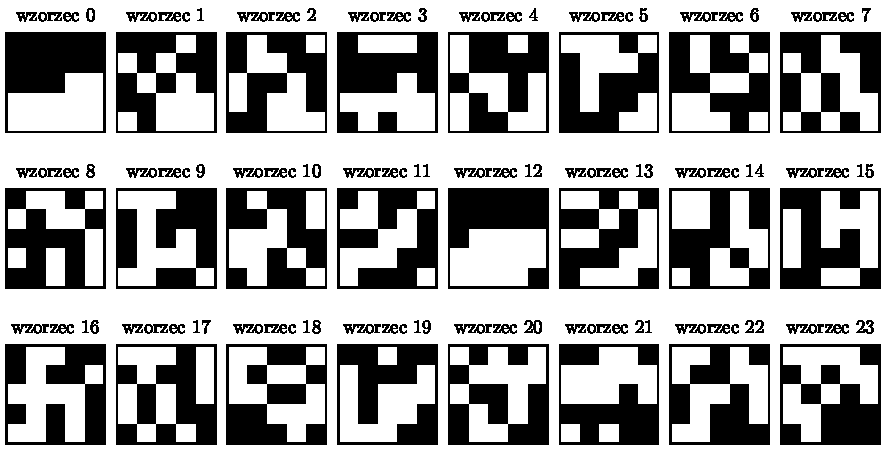
\includegraphics[width=\textwidth]{stable-5x5/figures/sample.pdf}
    \caption{Przykładowe elementy zbioru $S_u$ dla $u = (1, \ldots, 1, 2)$. Współrzędna $u_{25} = 2$ odpowiada prawemu dolnemu pikselowi.}
    \label{fig:stabilne-probka}
\end{figure}

\subsection{Oscylacja}
\label{sec:oscylacja}

Cykl długości 2 powstaje, gdy pole lokalne ma w każdym pikselu znak przeciwny do stanu (rozdział~\ref{sec:stany-pozorne}). Przy regule Hebba można to uzyskać dzięki wyzerowanej przekątnej. Z~\eqref{eq:hebb} pole w stanie $x$ wynosi
\begin{equation}
    h = \frac{1}{N} \sum_{\mu=1}^{p} \xi^\mu \left(\xi^\mu \cdot x\right) - \frac{p}{N} x.
    \label{eq:pole-cykl}
\end{equation}
Gdy $x$ ma małe nakładanie ze wszystkimi wzorcami, przeważa drugi składnik i w kroku synchronicznym zmieniają się wszystkie piksele. W stanie $-x$ pole ma przeciwny znak, więc sieć wraca do $x$.

Jako zbiór uczący wybrano cztery kształty T, L, H i +, a jako wejście szachownicę z czarnymi narożnikami (Rysunek~\ref{fig:oscylacja}). Szachownica ma iloczyn skalarny 1 z każdym kształtem, więc według~\eqref{eq:pole-cykl} jej pole wynosi $h = \frac{1}{25} \left(\sum_\mu \xi^\mu - 4 x\right)$. W żadnym pikselu wszystkie cztery kształty nie mają tej samej wartości co szachownica, więc $x_i h_i < 0$ w każdym pikselu, a najmniejsza wartość $\lvert x_i h_i \rvert$ wynosi $2/25$. Po jednym kroku synchronicznym zmienia się wszystkie 25 pikseli i sieć przechodzi w negację szachownicy, a po następnym wraca do stanu początkowego. Oba stany mają tę samą dodatnią energię \num{1.92}. W trybie asynchronicznym zmiana dowolnego piksela obniża energię o $2 \lvert x_i h_i \rvert$ (rozdział~\ref{sec:model}), więc szachownica jest maksimum lokalnym energii, a ta sama sieć dochodzi do punktu stałego.

\begin{figure}[H]
    \centering
    \begin{minipage}[t]{0.6\textwidth}
        \vspace{0pt}
        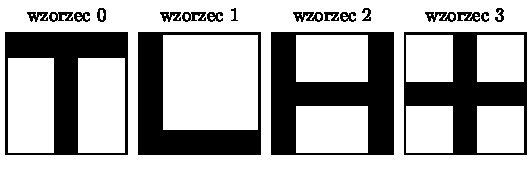
\includegraphics[width=\textwidth]{cycle/figures/patterns.pdf}
    \end{minipage}%
    \hspace{0.04\textwidth}%
    \begin{minipage}[t]{0.3\textwidth}
        \vspace{0pt}
        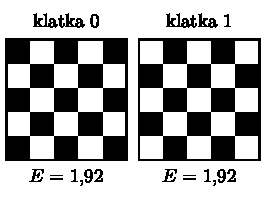
\includegraphics[width=\textwidth]{cycle/figures/frames.pdf}
    \end{minipage}
    \caption{Oscylacja w trybie synchronicznym. Lewy wykres: zbiór uczący reguły Hebba. Prawy wykres: szachownica podana na wejście (klatka 0) i jej negacja po jednym kroku (klatka 1).}
    \label{fig:oscylacja}
\end{figure}
